\chapter{Optimization, Classification, and Regularization}

Once a model family has been fixed, the next question is how to train it reliably and how to keep it from merely memorizing the training set. This chapter connects empirical risk minimization, gradient-based optimization, probabilistic classification, and regularization.

\section{Empirical risk minimization}

For data $(\vec{x}_i, y_i)_{i=1}^{N}$ and parameters $\wvec$, the training objective is usually written as
\[
  R_{\mathrm{emp}}(\wvec)
  =
  \frac{1}{N}\sum_{i=1}^{N} \ell(\wvec;\vec{x}_i,y_i).
\]
If regularization is added, one instead minimizes
\[
  J(\wvec) = R_{\mathrm{emp}}(\wvec) + \lambda \Omega(\wvec).
\]

\begin{aside}[Why this matters]
The empirical risk is only a sample average. Minimizing it is sensible only if low training loss is informative about low future loss. The rest of the chapter explains why that can fail and what one does about it.
\end{aside}

\section{Gradient-based optimization}

Gradient descent updates parameters by
\[
  \wvec_{t+1} = \wvec_t - \eta_t \nabla J(\wvec_t).
\]
The main regimes differ only in how the gradient is estimated:
\begin{itemize}
  \item \textbf{batch gradient descent}: use all samples for each update,
  \item \textbf{stochastic gradient descent}: use one sample at a time,
  \item \textbf{mini-batch methods}: use a small subset of samples per update.
\end{itemize}

Mini-batches are the practical default because they trade variance against compute well. Momentum, adaptive step sizes, and methods such as Adam improve this baseline by smoothing noisy gradients and scaling updates per parameter \parencite{goodfellow2016deep,bishop2006prml}.

\section{Probabilistic classification}

In multi-class classification, a network often outputs logits $z_k(\vec{x})$ that are converted to probabilities by the softmax map
\[
  p(C_k \mid \vec{x}, \wvec)
  =
  \frac{\exp z_k(\vec{x})}{\sum_j \exp z_j(\vec{x})}.
\]
If the target is one-hot encoded as $y_k \in \{0,1\}$ with $\sum_k y_k = 1$, the cross-entropy loss becomes
\[
  L(\wvec)
  =
  -\sum_k y_k \log p(C_k \mid \vec{x}, \wvec).
\]

\begin{keyequation}[Softmax plus cross-entropy]
\[
L(\wvec)
=
-\sum_k y_k \log p(C_k \mid \vec{x}, \wvec)
\]
\tcblower
The loss is small only when the model assigns high probability to the correct class. Classification is therefore turned into likelihood maximization over a categorical model.
\end{keyequation}

The important conceptual shift is that the network no longer outputs only a label. It outputs a distribution over labels. That makes uncertainty explicit and allows training by a smooth differentiable objective.

\section{Generalization, bias, and variance}

A model may achieve low training error and still fail on new data. The missing quantity is the \emph{generalization error}, the expected loss on unseen samples from the same population.

\begin{figure}[t]
\centering
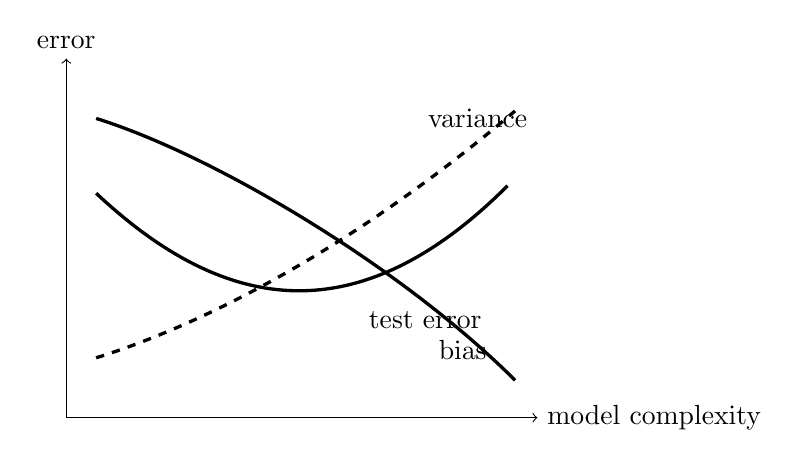
\begin{tikzpicture}[scale=0.95]
  \draw[->] (0,0) -- (6.3,0) node[right] {model complexity};
  \draw[->] (0,0) -- (0,4.8) node[above] {error};
  \draw[very thick] (0.4,4.0) .. controls (2.0,3.5) and (4.5,2.0) .. (6.0,0.5);
  \draw[very thick, dashed] (0.4,0.8) .. controls (2.0,1.3) and (4.0,2.4) .. (6.0,4.1);
  \draw[very thick] (0.4,3.0) .. controls (2.0,1.5) and (3.8,1.0) .. (5.9,3.1);
  \node at (5.3,0.9) {bias};
  \node at (5.5,4.0) {variance};
  \node at (4.8,1.3) {test error};
\end{tikzpicture}
\caption{Increasing model complexity reduces bias but increases variance. The test error is minimized between underfitting and overfitting.}
\end{figure}

The standard vocabulary is:
\begin{itemize}
  \item \textbf{underfitting}: the model class is too rigid,
  \item \textbf{overfitting}: the model fits noise in the sample,
  \item \textbf{bias}: systematic error from limited flexibility,
  \item \textbf{variance}: sensitivity to the specific training sample.
\end{itemize}

\section{Regularization and validation}

Regularization adds inductive bias that prefers simpler explanations. Common tools are:
\begin{itemize}
  \item \textbf{weight decay}: penalize large weights with $\Omega(\wvec)=\lVert \wvec \rVert_2^2$,
  \item \textbf{early stopping}: stop when validation error ceases to improve,
  \item \textbf{cross-validation}: estimate out-of-sample performance by repeated train/validation splits,
  \item \textbf{train/validation/test separation}: use different subsets for fitting, model selection, and final evaluation.
\end{itemize}

\begin{aside}[Geometric intuition of weight decay]
Without regularization, many parameter vectors may fit the same sample. Weight decay prefers solutions that stay near the origin, which often correspond to smoother and less brittle decision rules.
\end{aside}

The chapter-level lesson is simple: training is not only about descending a loss surface. It is about finding parameters that both fit the observed sample and remain credible beyond it.
